	\synctex=1
	\documentclass[a4paper,11pt,svgnames]{book}
	
	\usepackage[utf8x]{inputenc}
	\usepackage{mathtools}
	\usepackage{thesis}
	\usepackage{calc}
	\usepackage{float}
	\usepackage{acronym}
	
	% \setlength{\marginparwidth}{2cm}
	% \setlength{\voffset}{-0.25in}
	% \setlength{\parskip}{0.1in}
	
	%\includeonly{5-architecture}
	%\includeonly{6-use-case}
	
	%\usepackage{draftwatermark}
	%\SetWatermarkScale{4}
	\usepackage{subfig}
	 \usepackage{listings}
	  \usepackage{courier}
	 \lstset{
	 		 basicstyle=\footnotesize\ttfamily,
	         numbers=none,               % Ort der Zeilennummern
	         numberstyle=\tiny,          % Stil der Zeilennummern
	         %stepnumber=2,               % Abstand zwischen den Zeilennummern
	         numbersep=5pt,              % Abstand der Nummern zum Text
	         tabsize=2,                  % Groesse von Tabs
	         extendedchars=true,         %
	         breaklines=true,            % Zeilen werden Umgebrochen
	         keywordstyle=\color{red},
	    	 frame=single,         
	 %        keywordstyle=[1]\textbf,    % Stil der Keywords
	 %        keywordstyle=[2]\textbf,    %
	 %        keywordstyle=[3]\textbf,    %
	 %        keywordstyle=[4]\textbf,   \sqrt{\sqrt{}} %
	         stringstyle=\color{white}\ttfamily, % Farbe der String
	         showspaces=false,           % Leerzeichen anzeigen ?
	         showtabs=false,             % Tabs anzeigen ?
	         belowcaptionskip=5pt, 
	         xleftmargin=2em, 
	         xrightmargin=0.8em,
	         %backgroundcolor=\color{lightgray},
	         showstringspaces=false      % Leerzeichen in Strings anzeigen ?        
	 }
	 \lstloadlanguages{% Check Dokumentation for further languages ...
	         %[Visual]Basic
	         %Pascal
	         %C
	         %C++
	         %XML
	         %HP
	         Java
	 }
	 
	%\usepackage{xcolor}
	\usepackage[usenames,dvipsnames,table]{xcolor}
	\usepackage{todonotes}
	
	\colorlet{punct}{red!60!black}
	\definecolor{background}{HTML}{FFFFFF}
	\definecolor{delim}{RGB}{20,105,176}
	\colorlet{numb}{magenta!60!black}
	
	\lstdefinelanguage{json}{
	    basicstyle=\scriptsize\ttfamily,
	    numbers=left,
	    numberstyle=\scriptsize,
	    stepnumber=1,
	    numbersep=4pt,
	    showstringspaces=false,
	    breaklines=true,
	    frame=lrtb,
	    backgroundcolor=\color{background},
	    literate=
	     *{0}{{{\color{numb}0}}}{1}
	      {1}{{{\color{numb}1}}}{1}
	      {2}{{{\color{numb}2}}}{1}
	      {3}{{{\color{numb}3}}}{1}
	      {4}{{{\color{numb}4}}}{1}
	      {5}{{{\color{numb}5}}}{1}
	      {6}{{{\color{numb}6}}}{1}
	      {7}{{{\color{numb}7}}}{1}
	      {8}{{{\color{numb}8}}}{1}
	      {9}{{{\color{numb}9}}}{1}
	      {:}{{{\color{punct}{:}}}}{1}
	      {,}{{{\color{punct}{,}}}}{1}
	      {\{}{{{\color{delim}{\{}}}}{1}
	      {\}}{{{\color{delim}{\}}}}}{1}
	      {[}{{{\color{delim}{[}}}}{1}
	      {]}{{{\color{delim}{]}}}}{1},
	}
	    %\DeclareCaptionFont{blue}{\color{blue}} 
	
	  %\captionsetup[lstlisting]{singlelinecheck=false, labelfont={blue}, textfont={blue}}
	  \usepackage{caption}
	%\DeclareCaptionFont{white}{\color{white}}
	%\DeclareCaptionFormat{listing}{\colorbox[HTML]{6DBAFF}{\parbox{\textwidth}{\hspace{5pt}#1#2#3}}}
	
	\DeclareCaptionFont{white}{\color{white}}
	\DeclareCaptionFormat{listing}{\colorbox{gray}{\parbox{\textwidth-20pt}{#1#2#3}}\vspace{0.01cm}}
	\captionsetup[lstlisting]{format=listing,labelfont=white,textfont=white}
	
	\captionsetup[lstlisting]{format=listing,labelfont=white,textfont=white, singlelinecheck=false, margin=0pt, font={bf,footnotesize}}
	
	
	\usepackage{url}
	
	%\usepackage[spanish]{babel}
	%\usepackage[T1]{fontenc}
	\usepackage{tabularx}
	\usepackage{graphicx}
	%\usepackage[usenames,dvipsnames,table]{xcolor}
	\usepackage{verbatim}
	\usepackage[section]{placeins}
	\usepackage{listings}
	%\bibliographystyle{unsrt}
	
	
	\newcommand{\authorname}{Juan Álvarez Fernández del Vallado}
	\newcommand{\tfgtitle}{Sarcasm detetction on Twitter}
	\newcommand{\tfgtitlees}{Detección de Sarcasmo en Twitter}
	\newcommand{\supervisor}{Carlos Angel Iglesias Fernández}
	\newcommand{\fecha}{Enero 2019}
	
	\usepackage[pdftex,
	    pdfauthor={\authorname},
	            pdftitle={\tfgtitle},
	            pdfsubject={Bachelor Final Project},
	            pdfproducer={PDFTex},
	            colorlinks=true,linkcolor=black,citecolor=black,urlcolor=black,hypertexnames=false]{hyperref}
	\usepackage{cleveref}
	%\usepackage{longtable}
	\setcounter{secnumdepth}{3}
	
	\usepackage{framed}
	
	%lstlisting
	\usepackage{listings}
	
	\lstdefinelanguage{JavaScript}{
	  keywords={typeof, new, true, false, catch, function, return, null, catch, switch, var, if, in, while, do, else, case, break},
	  keywordstyle=\color{blue}\bfseries,
	  ndkeywords={class, export, boolean, throw, implements, import, this},
	  ndkeywordstyle=\color{darkgray}\bfseries,
	  identifierstyle=\color{black},
	  sensitive=false,
	  comment=[l]{//},
	  morecomment=[s]{/*}{*/},
	  commentstyle=\color{purple}\ttfamily,
	  stringstyle=\color{red}\ttfamily,
	  morestring=[b]',
	  morestring=[b]"
	}
	
	\definecolor{darkblue}{rgb}{0.0,0.0,0.6}
	
	\lstdefinestyle{listXML}{language=XML, basicstyle=\ttfamily\diny, extendedchars=true,  belowcaptionskip=5pt,xleftmargin=0.4em, xrightmargin=0.3em, numbers=none, frame=single, breaklines=true, breakatwhitespace=true, breakindent=0pt, emph={}, emphstyle=\color{red}, basicstyle=\small\ttfamily, columns=fullflexible, showstringspaces=false, commentstyle=\color{gray}\upshape,
	morestring=[b]",
	morecomment=[s]{<?}{?>},
	morecomment=[s][\color{orange}]{<!--}{-->},
	keywordstyle=\color{cyan},
	stringstyle=\color{black},
	tagstyle=\color{darkblue},
	morekeywords={xmlns,version,type}
	}
	
	
	
	\lstdefinestyle{mono}{
	   framesep=8px,
	   extendedchars=true,
	   basicstyle=\ttfamily,
	   showstringspaces=false,
	   showspaces=false,
	   tabsize=2,
	   breaklines=true,
	   showtabs=false,
	   xleftmargin=8pt,
	   xrightmargin=8pt
	}
	
	
	\lstdefinestyle{commands}{
	   framesep=8px,
	   extendedchars=true,
	   basicstyle=\ttfamily,
	   showstringspaces=false,
	   showspaces=false,
	   tabsize=2,
	   breaklines=true,
	   showtabs=false,
	   xleftmargin=8pt,
	   xrightmargin=8pt
	}
	
	\lstdefinestyle{consola}
	   {basicstyle=\scriptsize\ttfamily,
	    backgroundcolor=\color{white},
	    frame=lrtb,
	    numbers=none,
	    xleftmargin=4pt,
	    xrightmargin=4pt
	   }
	
	% Allows to change the color of chapter headers
	\definecolor{chapterdetails}{HTML}{00a9e0}
	
	% \usepackage[sf,bf]{titlesec}
	% \titleformat{\chapter}[display]
	%   {\normalfont\Large\sffamily\raggedleft}
	%   {\vspace{5cm}\MakeUppercase{\chaptertitlename}%
	%     \rlap{ \resizebox{!}{1.5cm}{\thechapter} \color{chapterdetails}\rule{5cm}{1.5cm}}}
	%   {10pt}{\Huge}[{\color{chapterdetails}\titlerule[0.8mm] }]
	% \titlespacing*{\chapter}{0pt}{30pt}{20pt}
	
	\usepackage[sf,bf]{titlesec}
	\titleformat{\chapter}[display]
	  {\normalfont\Large\sffamily\raggedleft}
	  {\vspace{5cm}\MakeUppercase{\chaptertitlename}%
	    \rlap{ \resizebox{!}{1.5cm}{\thechapter} \color{chapterdetails}\rule{5cm}{1.5cm}}}
	  {10pt}{\Huge}[{\color{chapterdetails}\titlerule[0.8mm] }]
	\titlespacing*{\chapter}{0pt}{30pt}{20pt}
	
	%\titleformat{\section}{\large\sffamily\bfseries}{\thesection}{1em}{}
	
	
	\newenvironment{chapterintro}
	{% This is the begin code
	\large\it
	}
	{% This is the end code
	}
	
	
	% Tick symbols
	\newcommand{\tickYes}{\checkmark}
	\newcommand{\tickNo}{\hspace{1pt}\ding{55}}
	% Fancy header
	\usepackage{fancyhdr}
	%Fancy chapter cover style
	
	
	% Fancy box
	\usepackage{fancybox} 
	\setlength{\fboxrule}{1 pt} \setlength{\fboxsep}{10pt} \setlength{\shadowsize}{3pt}
	
	%Sky color definition
	
	%% Portada
	\usepackage{eso-pic,graphicx}
	% \usepackage{tikz}
	% \usepackage[top=0cm, bottom=0cm, outer=0cm, inner=0cm]{geometry}
	
	
	\begin{document}
	\acrodef{nlp}[NLP]{Natural Language Processing}
	\acrodef{ml}[ML]{Machine Learning}
	\acrodef{nltk}[NLTK]{Natural Language Toolkit}
	\acrodef{svm}[SVM]{Support Vector Machine}
	\acrodef{json}[JSON]{Javascript Object Notation}
	\acrodef{rf}[RF]{Random Forests}
	\acrodef{TAS}[TAS]{Task Automation Service}
	\acrodef{lda}[LDA]{Latent Dirichlet Allocator}
	\acrodef{tfidf}[TFIDF]{Frequency Inverse Document Frequency}
	\acrodef{nb}[NB]{Naive Bayes Classifier}
	\acrodef{pdf}[PDF]{Probability Density Function}
	\acrodef{gs}[GS]{Grid Search}
	\acrodef{tp}[TP]{True Positive}
	\acrodef{tn}[TN]{True Negative}
	\acrodef{fp}[FP]{False Positive}
	\acrodef{fn}[FN]{False Negative}
	\acrodef{knn}[k-NN]{K-Nearest Neighbors}
	\acrodef{lr}[LR]{Logistic Regression}
	\newcommand\litem[1]{\item{\bfseries #1 }}
	\renewcommand{\arraystretch}{1.5} %Makes tables less crammed
	
	\newcommand\headcell[1]{%
	  \multicolumn{1}{|c|}{\cellcolor{DodgerBlue}\bfseries\sffamily\textcolor{white}{#1}}
	}
	
	
	
	%Cuadros por tablas
	%\renewcommand{\listtablename}{Tables Index}
	%\renewcommand{\tablename}{Table} 
	
	% \renewcommand{•}{•}*{\lstlistingname}{List of X}
		
	\pagenumbering{Roman}
	
	\pagestyle{empty}
% \tikz[remember picture,overlay] \node[opacity=1,inner sep=0pt] at (current page.center){
\includegraphics[height=\paperheight]{img/portada.png}};

\vspace*{5.5cm}

\begin{center}

{\Large\rm \textbf{ GRADO EN INGENIERÍA DE TECNOLOGÍAS Y\\
SERVICIOS DE TELECOMUNICACIÓN\\}}

\vspace{1.0cm}

{\Large\rm \textbf{TRABAJO FIN DE GRADO}}

\vspace{2cm}

{\Large\rm\textbf{\tfgtitle}}

\vspace*{\fill}

{\Large\rm\textbf{Juan Álvarez Fernández del Vallado}}

{\Large \textbf{2018}}
\vspace{1.0cm}
\end{center}
\AddToShipoutPictureBG*{
\includegraphics[width=\paperwidth,height=\paperheight]{img/portada.png}}

\cleardoublepage
\thispagestyle{empty}
\vspace*{3\baselineskip}
{\large{\bf TRABAJO DE FIN DE GRADO}}
\vspace{0.5cm}

\begin{rm}
\begin{tabular}{p{3cm}p{10cm}}
\textbf{Título: } & \tfgtitlees \\ 
\textbf{Título (inglés):} & \tfgtitle \\ 
\textbf{Autor:} & Juan Álvarez Fernández del Vallado \\ 
\textbf{Tutor:} & Carlos Ángel Iglesias Fernández \\ 
\textbf{Departamento:} & Departamento de Ingeniería de Sistemas Telemáticos \\ 
\end{tabular} \end{rm} \vspace{1cm}

{\large{\bf MIEMBROS DEL TRIBUNAL CALIFICADOR}} \vspace{0.5cm}

\begin{rm}
\begin{tabular}{p{3cm}p{10cm}}
\textbf{Presidente:} & -----\\
\textbf{Vocal:} & -----\\
\textbf{Secretario:} & -----\\
\textbf{Suplente:} & -----
\end{tabular}
\end{rm}
\vspace{1cm}

{\large{\bf FECHA DE LECTURA:}}
\vspace{1cm}

{\large{\bf CALIFICACIÓN:}}
\pagestyle{empty}
\cleardoublepage
\vspace*{\baselineskip}
\begin{center}
	{\LARGE\rm\textbf{UNIVERSIDAD POLITÉCNICA DE MADRID}\\
	\vspace{1.0cm}
	 ESCUELA TÉCNICA SUPERIOR DE\\ INGENIEROS DE TELECOMUNICACIÓN
	  }  \\

	 {\Large\rm Departamento de Ingeniería de Sistemas Telemáticos\\}  \\

\begin{figure}[!htbp]
	\centering
    
\includegraphics[width=0.7\textwidth]{img/logo_etsit.jpg}

\end{figure}
	\vspace{1.0cm}
	{\LARGE\rm TRABAJO DE FIN DE GRADO\\
	\vspace{2.0cm}
    \tfgtitle
	 \vspace{0.5cm}}
	 
	 \vspace{1.0cm}
     \Large\rm\textbf{\author}\\
	 \vspace{1.0cm}
     \fecha
\end{center}  

%\cleardoublepage
%
%\begin{tabular}{p{10cm}p{4cm}}
%&\\
%&\\
%&\\
%&\\
%&\\
%&\\
%&\\
%&\\
%&\\
%&\emph{Write cool quote here}\\
%&\\
%\end{tabular}
	\cleardoublepage
\phantomsection
\chapter*{Resumen}
\addcontentsline{toc}{chapter}{Resumen}
 La aparición de la red social Twitter en el año 2006 llevó consigo un tremendo empujón a la Revolución Digital que ya se estaba viviendo desde finales del siglo 20. Como resultado, a día de hoy se twittean unos 6000 tweets cada segundo. Se estima que para el año 2020 la red social Twitter contará con 275 millones de usuarios en todo el mundo. Tal es la popularidad de Twitter que casi el 74\% de sus usuarios usan Twitter a diario para consultar las noticias del día a día. Se podría decir que la Revolución Digital ha convertido a Twitter en una parte de nuestras vidas. Es por estas razones que este proyecto tiene como objetivo desarrollar un clasificador con la habilidad de detectar el sarcasmo en textos cortos, como en tweets.\par
 El propósito de este proyecto es conseguir la detección automatizada de sarcasmo. El principal desafío a tener en cuenta es la detección de emociones en frases que contienen sentimiento. Para abordar este enorme reto, se ha diseñado un clasificador que posee tecnologías de~\ac{ml}, el cuál podrá aprender a detectar sarcasmo. También han sido necesarias herramientas capaces de procesar lenguaje natural (\ac{nlp}). Con el fin de obtener unos parámetros adecuados en el clasificador se han llevado a cabo pruebas para ver que características aportan información relevante sobre el sarcasmo al clasificador. Las mas notables fueron los ngramas, las características léxicas y~\ac{lda}. Además, se ha llevado a cabo un~\ac{gs} con el propósito de buscar los parámetros óptimos del clasificador. Esto ha consistido en obtener el F1 score (medida de cómo de bueno es el clasificador) para cada permutación de una tabla de parámetros a probar. Una vez se obtuvieron los mejores parámetros, la plataforma senpy fue usada para dar una interfaz intuitiva en la que un usuario puede introducir texto y el clasificador indica si el texto tiene sarcasmo.\par
 Para terminar, los resultados obtenidos han oscilado, presentando un mínimo F1 score de $90.22$\% y un máximo de $96.68$\%. Esta diferencia se debe a las diferentes características extraídas y a los parámetros usados. En realidad, cuantas mas características son extraídas, peor es la capacidad del clasificador de generalizar. Y esto se traduce en que la precisión del clasificador disminuye. Este fenómeno también se conoce como overfitting.
\vfill
\textbf{Palabras clave:} Sarcasmo, Twitter, Machine Learning, Big Data, Python, NLP, Detección de Sarcasmo, Sentimientos, Emociones y Análisis. 
	\cleardoublepage
\phantomsection
\chapter*{Abstract}
\addcontentsline{toc}{chapter}{Abstract}


\vfill
\textbf{Keywords:} 
	% \cleardoublepage
\phantomsection
\addcontentsline{toc}{chapter}{Acknowledgement}

\begin{center}
\textbf{\large Acknowledgement}
\end{center}

Acknowledgement
	\cleardoublepage
\phantomsection
\chapter*{Agradecimientos}
\addcontentsline{toc}{chapter}{Agradecimientos}

A Gauss
	\cleardoublepage
\phantomsection
\addcontentsline{toc}{chapter}{Contents} % para que aparezca en el indice de 
\tableofcontents % indice de contenidos


\cleardoublepage
\phantomsection
\addcontentsline{toc}{chapter}{List of Figures} % para que aparezca en el indice de contenidos
\listoffigures % indice de figuras
%\cleardoublepage
%\phantomsection
%\addcontentsline{toc}{chapter}{List of Tables} % para que aparezca en el indice de contenidos
%\listoftables % indice de tablas

\cleardoublepage
	
	
	%Header style
	\pagestyle{fancy}
	\fancyhf{}
	\fancyhead[RO]{\sffamily \slshape \rightmark}
	\fancyhead[LE]{\sffamily \slshape \leftmark}
	%\renewcommand{\footrulewidth}{0.4pt} % grosor de la línea del pie
	\fancyfoot[OR,EL]{\rmfamily \thepage} % texto derecha del pie
	\pagenumbering{arabic}
	
	\chapter{Introduction}

\section{Context}
The emergence of the social network Twitter in 2006 led to a tremendous boost of the Digital Revolution taking place since the end of the 20th century. As a result, there are on average at least 6000 tweets being tweeted every second. It is estimated that by 2020 the number of users on Twitter will increase up to 275 million users worlwide~\cite{twitter1}. Twitter has become so popular that roughly 74\% of all the Twitters' users claim to use the social network as a source to get the daily news~\cite{twitter2}. One could say that Twitter has become part of our lives and he would not be far from the truth.\par

 Combining the data allocated in the Twitter database with mathematical models can create insights that we are not capable of imagining. Moreover, the Twitter API offers the possibility of making topic-based queries, allowing the developer to get an enormous amount of data from almost any subject. Therefore, Twitter is like a gold mine of data. Additionally, spatial data can also be obtained by using the Twitter API. This can be very interesting if the developer wants to see what is the feeling of the people from an area towards a certain product or company. \par
According to~\cite{shayaa2018sentiment}, the world has already generated 1~\ac{zb} of data and it is supposed to increase up to 44~\ac{zb} by 2020. The 44~\ac{zb} will contain at least half of lexical data, coming from social networks like Facebook, Twitter and instant messaging platforms. Furthermore, it is expected that this humongous amount of data will continuously grow due to the influx of digital technologies that have already sprung up in the digital era.\par
Since an enormous amount of text data has arisen, there is a great need to give some insight to raw data. In that context, text mining uses~\ac{nlp} and~\ac{ml} techniques to process the data. Usually, text analysis is conducted for two purposes~\cite{shayaa2018sentiment}. The first purpose is to analyze peoples' sentiment on an issue. The second purpose is to evaluate peoples' opinion and sentiment on a product or topic.\par
Finally, to give a glimpse of the results achieved, the senpy engine was implemented to provide a framework where a user could insert a short text and the classifier could detect whether or not the text is sarcastic.
\section{Project goals}
The main objective of this project is to define a classifier capable of detecting sarcasm in texts, particularly in tweets. To do so, the following challenges shall be overcome:

\begin{itemize}

\item  \textit{Tweet body retrieval}: The data provided will only contain tweets id and a sarcastic indicator. Hence, software capable of downloading the body of the tweets is required.
\item \textit{Dataset preprocessing}: To combine different datasets and encode categorical values, a preprocessing stage is mandatory.
\item \textit{Feature extracion}: If the mathematical classifier is to learn from the body of the tweets, a feature extraction process is required.
\item \textit{Model creation}: Create classification models using different mathematical learning techniques.
\item \textit{Optimization}: For the classifier to be optimal, the model will have the best parameters, most relevant features and greatest mathematical learning technique.
\item \textit{Senpy implementation}: Implement the optimum classifier in the senpy engine as a plugin to create a framework where a user can insert a short text and the classifier detects whether or not the text is sarcastic.

\end{itemize}

\section{Structure of this document}
In this section, we provide a brief overview of the chapters included in this document. The structure is as follows:

\textbf{\textit{Chapter 1}} discusses the context wherein this project is located and gives an insight into the topics that this project will cover.

\textbf{\textit{Chapter 2}} describes what are the results already achieved in similar works. Serves as a benchmark.

\textbf{\textit{Chapter 3}} from a generic perspective explains the technologies chosen to create the model.

\textbf{\textit{Chapter 4}} analyzes extensively how are the technologies from~\cref{chap:entech} implemented and shows the results achieved.

\textbf{\textit{Chapter 5}} finalizes the project showing the conclusions drawn and shows what were the problems faced.

	\chapter{State of the Art}
\label{chap:enabling_technologies}
This chapter will serve as a compilation of past work in automatic sarcasm detection.
Firstly, a brief introduction to the main learning technologies used for text-based learning will be given. Moreover, an analysis of automatic sarcasm detection will be briefed. Finally, the main issues found in automatic sarcasm detection shall be overviewed.

\section{Introduction}
Sarcasm detection is an important component for~\ac{nlp} very relevant to natural language understanding, dialogue systems and text mining~\cite{khodak2017large}.\\ The perspective followed in this chapter is merely to give a glimpse to the reader of the state-of-the-art technologies used by other researchers in this field. \\
The chapter will begin by defining sarcasm and its context. 
\section{Sarcasm} 
\subsection{Sarcasm Definition}
The Free Dictionary\footnote{www.thefreedictionary.com} defines sarcasm as a form of verbal irony that is intended to express contempt or ridicule. The subjective characteristic of sarcasm makes sarcasm very difficult to detect since a word may have a literal meaning and a sarcastic meaning. As a result, sarcasm automatic detection presents a big challenge~\cite{joshi2017automatic}. \\
Typically, sarcasm detection has been formulated as a classification problem. In that sense, given text, the goal is to predict whether or not the text is sarcastic. However, the big challenge is to label the text, since the classifier is supposed to distinguish between irony,  humour and other sentimental meanings.\\
In linguistics, sarcasm is a form of figurative language where the literal meaning of words does not hold, and instead, the opposite interpretation is intended. Sarcasm is a type of irony. 

\section{Dataset}

As a matter of a fact, the studies already done in automatic sarcasm detection depend entirely on the dataset. That is why it is convenient to divide them into three kinds~\cite{joshi2017automatic}:
\begin{itemize}
	\item \textit{Short texts}: The social network Twitter is extremely popular due to its popularity among users. It can serve as an example of short text since every tweet is restricted to not exceed a certain number of words. One approach to obtaining labels for the tweets is to manually mark them as sarcastic or non-sarcastic. Another approach is hashtag-based supervision. Hashtags can reveal when a tweet is labelled as sarcastic. By introducing the \textit{sarcasm} label, the author makes clear his intention to use sarcasm.  This allows the dataset to be bigger. Many works using this variation have been reported since its popularity has constantly grown. One of the problems with Twitter is the text length restriction. If the tweet length exceeds the tweet restriction limit, the author is going to be forced to introduce abbreviations to the words used. As a consequence, sarcasm detection is going to be harder since the words are not going to be correctly spelt.
	\item \textit{Long texts}: The information usually comes from reviews, posts, news, articles. Some of the popular platforms for sentiment analysis in long texts are imdb (for film critiques) and reddit. 
	\item \textit{Other data-sets}
\end{itemize}

It is noteworthy to mention the emphasis made on the Twitter social network since this project will be focusing on a Spanish set of tweets to detect sarcasm. Please note that this project will be developed for short texts. Hence, all the conclusions made are only valid for short texts.

\section{Approaches used for Sarcasm Detection}
\label{sec:sarcasmapproach}
In this section, several approaches used for detecting sarcasm will be discussed. In general, approaches for sarcasm detection can be classified into rule-based, statistical and deep learning-based approaches~\cite{joshi2017automatic}.
\subsection{Rule-based Approaches}
Rule-based approaches work by identifying sarcasm through a set of rules based upon evidence~\cite{joshi2017automatic}. The evidence is captured by using rules relying upon sarcasm. For instance, one rule can rely on Google to determine how likely that smile (emoticon) is while another rule can come from hashtag analysis. By identifying the hashtags present in a tweet, a sarcasm pattern could be found. If the sentiment detected in the tweet does not match with the hashtag, then that tweet is labelled as sarcastic.\\ Furthermore, one could find sarcasm if a positive verb happens in a negative situation phrase in a sentence. The problem here is extracting the set of negative situation phrases. This is also known as a rule-based approach.
\subsection{Feature sets}
This kind of approach used some of the technologies described below~\cite{joshi2017automatic}. In this project, there was a combination of features and learning algorithms but, in contrast, no deep learning technologies were implemented.
\begin{itemize}
	\item \textit{Features Used:} Most of these approaches use bag-of-words as features that have been found by statistical sarcasm detection. Apart from finding the features, some other works focus on designing pattern-based features, that are able to indicate sarcastic patterns on the corpus. The majority of the features used can be found in~\Cref{fig:featused}. To allow the classifier to spot sarcastic patterns, these pattern-based features take three real values: exact match, partial match and no match. Furthermore, pragmatic features, like emoticons, can also be considered. For the sake of simplicity, the contextual sarcastic features (i.e. features that depend on previous messages) are not considered in this project.
	\item \textit{Learning Algorithms:} A variety of classifiers have already experimented for sarcasm detection.~\acf{svm} is quite often present in sarcasm detection classification techniques. Moreover, many other works have used~\acf{lr},~\acf{nb} and Random Forests.
	\item \textit{Deep Learning-based Approaches:} Although nowadays deep learning has raised a lot of awareness, there are still few approaches reported for automated sarcasm detection. A similarity between word embeddings as features for sarcasm detection has been reported. This augments features based on similarity of word embeddings related to other word pairs and report an improvement on performance. Convolutional neural networks have also been implemented, reporting an improvement of $2\%$ in performance.
\end{itemize}
\begin{figure}
	\centering
	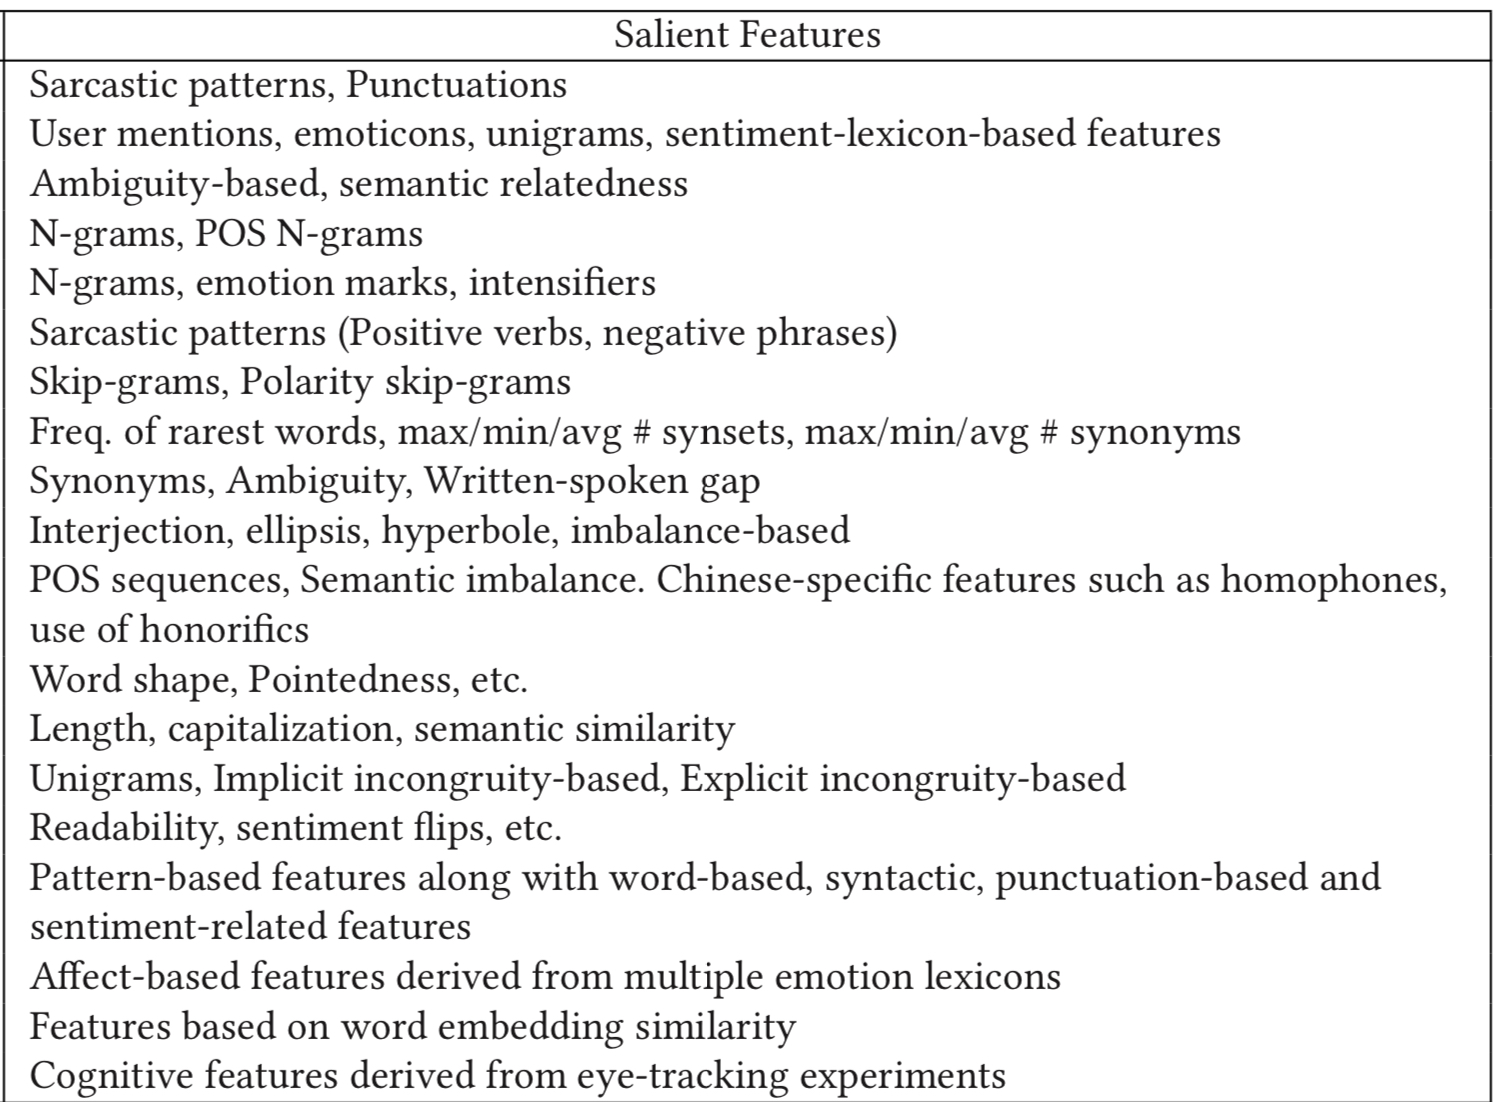
\includegraphics[scale=0.3]{img/features.jpeg}
	\caption{Features used for Statistical Classifiers~\cite{joshi2017automatic}}
	\label{fig:featused}
\end{figure}
To put it in a nutshell, different techniques for automatic sarcasm detection can be performed. Despite these numerous techniques, sarcasm automatic detection is difficult to detect since a word can have a literal meaning but also a sarcastic meaning that is not so easily labelled.

\section{Main Issues in Sarcasm Detection}
There are three main issues present in sarcasm automatic detection techniques~\cite{joshi2017automatic}:
\begin{itemize}
	\item \textit{Data:} Even though hashtag-based labelling can provide large-scale supervision, the quality of the dataset can be doubtful. For example, let us take the hashtag \textit{\#not} very often present in tweets. Is this supposed to express sarcasm in the sentence or is it simply used to express a negation? In most of the works, this problem is tackled by removing the \textit{\#not} in the pre-processing step and analyzing the sentence. However, this may as well not be the optimum solution. Another solution is to use as test set some manually labelled tweets and as train set a hashtag labelled set. 
	\item \textit{Features as Sentiment:} The question is how can sentiment be detected in a sentence? In the case of sarcasm, some answers have already been given. If a negative phrase occurs in a positive sentence then that sentence has most likely sarcasm. In a statistical classifier, surface polarity can be used as a feature of the tweet. To capture surface polarity one has to analyze two emotions: activation and pleasantness. This can lead to a $4\%$ improvement in the accuracy~\cite{joshi2017automatic}.
	\item \textit{Skewed Data-sets: }
	Sarcasm is hard to find in an expression. For that reason, skew is reflected in data-sets.
\end{itemize}

\section{Figures of Merit}
This section is committed to showing other past works in Sarcasm Detection for tweets. The decisive parameters shown in this section will be the F-measure.

\begin{itemize}
	\item Sarcasm Detection on Czech and English Twitter~\cite{ptavcek2014sarcasm}:
	\begin{itemize}
		\item \textit{Description}: This paper presents a \ac{ml} approach to sarcasm detection on Twitter in two languages - English and Czech. The classification was carried out by using~\ac{svm} classifiers and Maximum Entropy. Since only \ac{svm} has been implemented in this project, the latter will be discarded.
		\item \textit{Results:} F-measure (balanced dataset):~\textbf{0.947}. F-measure (unbalanced dataset):~\textbf{0.924}. Algorithm:~\textbf{\ac{svm}}
	\end{itemize}
	\item Irony detection in short texts\footnote{\url{ http://ru.ffyl.unam.mx/bitstream/handle/10391/4787/VII_CoLiCo_G_Jasso_Mesa_3_2015.pdf?sequence=2&isAllowed=y}}:
	\begin{itemize}
		\item \textit{Description}: This docuemnt summarizes the result of analyzing ironic tweets. The language is spanish.
		\item \textit{Results:} F-measure (balanced dataset):~\textbf{0.86}. F-measure (unbalanced dataset):~\textbf{0.82}. Algorithm:~\textbf{\ac{svm}}
	\end{itemize}
	
\end{itemize}
Moreover, in~\cite{joshi2017automatic} a table can be found with a collection of many other past works in sarcasm detection. However, the values on the table are not directly comparable, because different datasets and techniques have been used by the authors.\\
\begin{table}
	\centering
	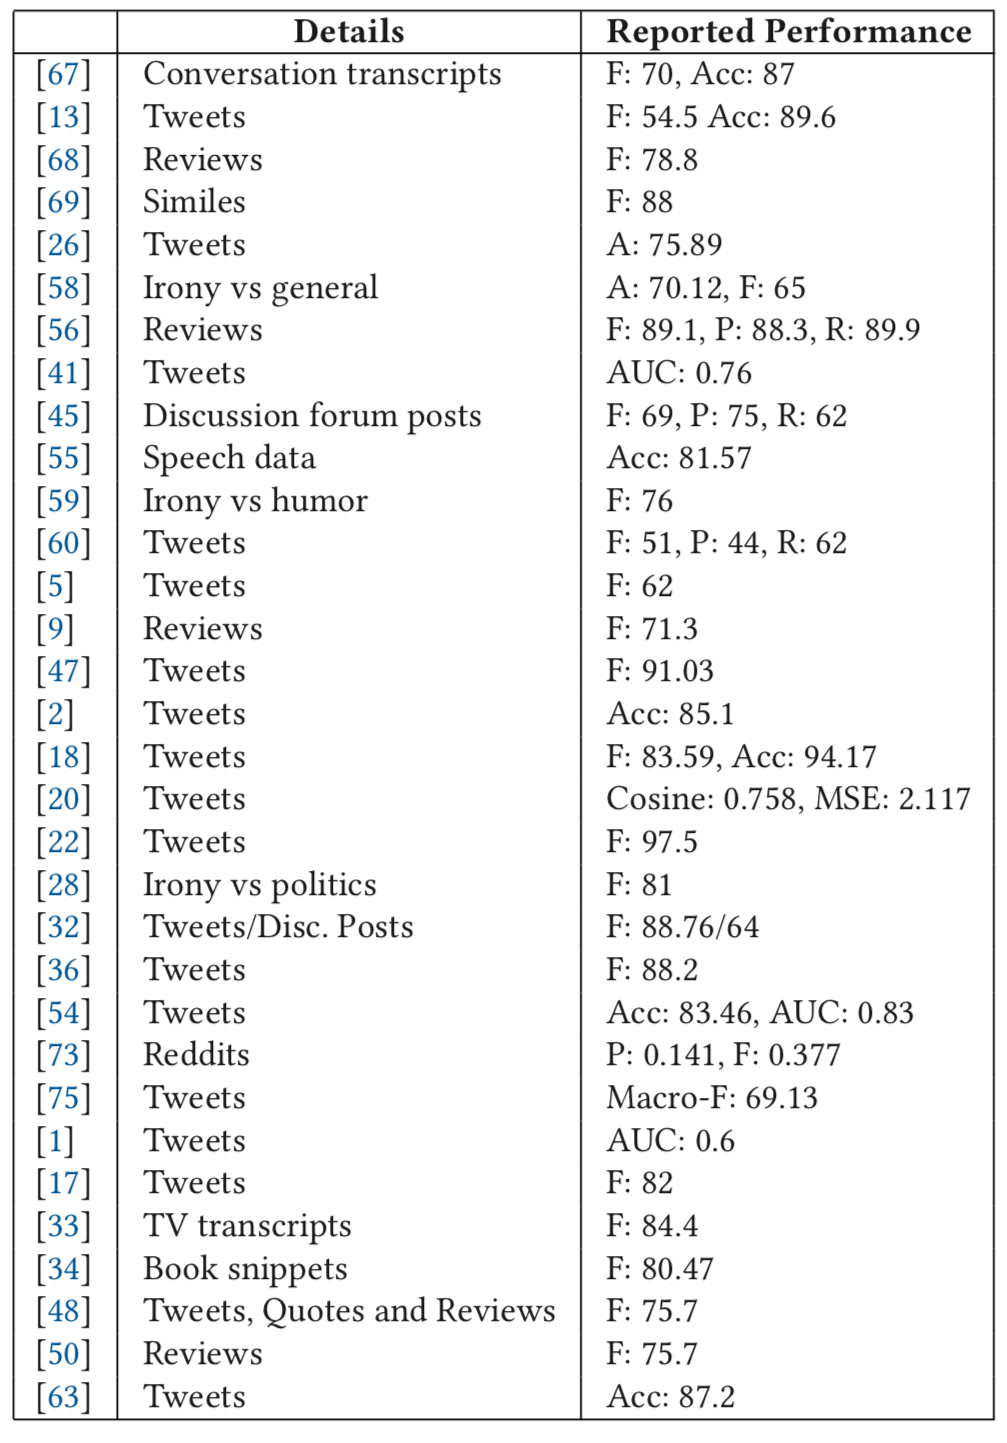
\includegraphics[scale=0.35]{img/performanceValues.jpeg}
	\caption{Performance Values of Sarcasm Detection; Precision/Recall/F-measures and Accuracy Values indicated in Percentages~\cite{joshi2017automatic}}
	\label{tab:performanceBench}
\end{table}
In the~\cref{tab:performanceBench} a compilation of performance values of sarcasm detection is shown.\\ 
The left column represents the citations used in the article~\cite{joshi2017automatic}. Therefore, they do not correspond to this projects' citations.\\
The middle column is expressing whether the dataset was composed of short texts, such as tweets, or other long texts, like reddits.\\
Finally, the third column shows the score achieved. To simplify, the F1 Score (in the table is represented as \textit{F}) will be considered the most relevant score. The average F1 Score is $76,771\%$. To compute the average, only tweets displaying a F1 Score in the table have been considered.\\
For more information on F1 Score see~\cref{sec:score}.
	\chapter{Enabling Technologies}
\label{chap:entech}


In this chapter, the technologies used to achieve this projects' objective shall be discussed.

\section{Introduction}\par
In this project two main technologies have been used:~\acf{nlp}  and~\acf{ml}. The implementation of these tools has been performed in a combined fashion. Furthermore, other technologies have also been used but they are less relevant than~\ac{nlp} and~\ac{ml}.
On the one hand, with~\ac{nlp} it was possible to transform words into tokens, find syntactical connections between tokens in the same tweet and, finally, construct a numerical vector. On the other hand,~\ac{ml} was very useful to construct a classifier, define a model and feed the vectors from the previous step into the model to make predictions.\par
In short, this is how the project was carried out. Both technologies will be extensively explained in the next sections.

\section{Natural Language Processing}
\ac{nlp} has a crucial role in this project since texts (tweets) is what this project is trying to deal with. Hence, the information that used to train the~\ac{ml} algorithm will come in the form of text. According to~\cite{bird2009natural}, at one extreme~\ac{nlp} could be as simple as counting word frequencies to compare different writing styles. At the other extreme,~\ac{nlp} involves "understanding" complete human utterances, at least to the extent of being able to give useful responses to them.\\
\begin{figure}
	\hspace{-1.45cm}
	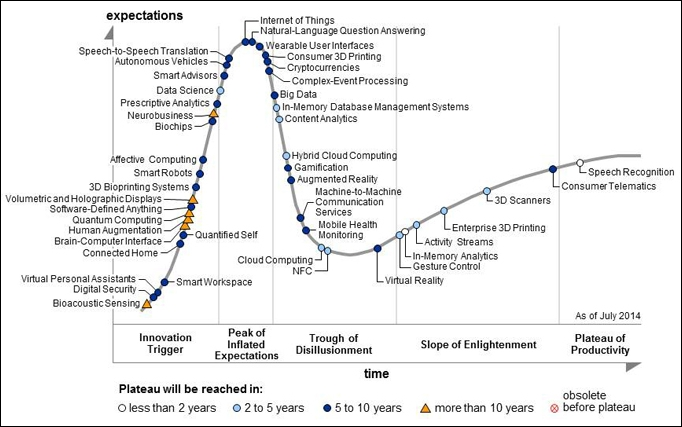
\includegraphics[]{img/nlp.jpg}
	\caption{Image is taken from~\url{http://www.gartner.com/newsroom/id/2819918}}
	\label{fig:nlptech}
\end{figure}
When the task is handling text,~\ac{nlp} is a very powerful tool. Such is the importance that many other applications that can be found everyday already implement it. \Cref{fig:nlptech} shows many emerging technologies that are using \ac{nlp} to provide their services.
Many other examples of \ac{nlp} applications are machine translation, optical character recognition, language detection, topic modelling and many more~\cite{stopwords}.

\label{sec:NLP}
\subsection{Natural Language Toolkit}
\subsubsection{Definition}
\ac{nltk} is a platform for building Python programs to work with human language data. It provides easy-to-use interfaces to over 50 corpora and lexical resources such as WordNet, along with a suite of text processing libraries for classification, tokenization, stemming, tagging, parsing, and semantic reasoning, wrappers for industrial-strength~\ac{nlp} libraries, and an active discussion forum~\footnote{https://www.nltk.org/}.\\
The following applications explained beneath belong to the~\ac{nltk} class.
\subsubsection{Application}
~\ac{nltk} has provided the following tools to this project:
\begin{itemize}
	
	\item \textit{Tokenizer}: A word (Token) is the minimal unit that a machine can understand and process. So any text string cannot be further processed without going through tokenization. Tokenization is the process of splitting the raw string into meaningful tokens~\cite{nltk}. In this project, tokenization was required to get the words containing a tweet. Furthermore, some of the tokens were removed since they do not add meaningful information (e.g. yo, a). These words belong to a stoplist provided by~\ac{nltk} for all supported languages~\cite{nltk}.
	\item \textit{Stemmer}: A stemmer is needed to remove affixes from a word, ending up with a stem. Stemming is frequently used for indexing words. Instead of storing all forms of a word, the algorithm stores only the stems, greatly reducing the size of the index while increasing retrieval accuracy~\cite{nltk}. Particularly, the SnowballStemmer was chosen because it supports stemming in 13 non-English languages, especially Spanish.
	\item \textit{Part-of-Speech tagging}:  A-part-of-Speech tagger (pos\_tag) indicates how a word is functioning within the context of a sentence~\cite{pos}. This part is crucial since a word can function in multiple ways and we would like to distinguish those cases. POS\_tagging has been achieved by collecting each word feature and building up a dictionary with the word features' stats. The word features offered by~\ac{nltk} are:
	\begin{enumerate}
		\item \textit{VERB}: Verbs (all tenses and modes)
		\item \textit{NOUN}: Nouns (common and proper)
		\item \textit{PRON}: Pronouns
		\item \textit{ADJ}: Adjectives
		\item \textit{ADV}: Adverbs
		\item \textit{ADP}: Adpositions (prepositions and postpositions)
		\item \textit{CONJ}: Conjunctions
		\item \textit{DET}: Determiners
		\item \textit{NUM}: Cardinal numbers
		\item \textit{PRT}: Particles or other function words
		\item \textit{X-other}: Foreign words, typos, abbreviations
		\item \textit{.}: Punctuation
	\end{enumerate}
\end{itemize}

The applications at the top of this section are more commonly known as the preprocessing part previously needed to any \ac{ml} application. Since there are plenty of tasks, they could be easily coordinated by using pipelines.\\ 
More information on how were these technologies implemented in the project can be found in~\cref{sec:preprocessing}.

\section{Machine Learning}
When it comes to defining models capable of learning from a text-based source, the two dominant technologies are~\acl{nlp} and~\acl{ml}. These two main technologies are concerned about how does the machine process human text~\cite{tfidf}. \\
Given data and the proper statistical techniques,~\ac{ml} automates analytical model building capable of recognizing patterns with the aim of making predictions and learning from the model. To be able to do so, a learning process is required.~\ac{ml} algorithms can be classified into three categories~\cite{dataclust}:
\begin{itemize}
	\item \textit{Regression}: Regression learning is predicting a continuous varying variable. Regression methods can be used to address classification and prediction models. To visualize a simple example of what regression is we can see the picture~\Cref{fig:regresion}.
	\begin{figure}
		\centering
		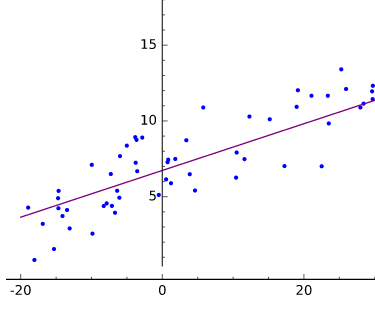
\includegraphics[scale=1.6]{img/regression.png}
		\caption{Linear regression plotted~\cite{tfidf}}
		\label{fig:regresion}
	\end{figure}
	\item \textit{Classification}: Classification is modeling based on delineating classes of output based on some set of input features. If regression gives us an outcome of "how much,” classification gives us an outcome of "what kind.”
	\item \textit{Clustering}: Clustering is an unsupervised learning technique that involves using a distance measure and iteratively moving similar items more closely together. At the end of the process, the items clustered most densely around $n$ centroids are considered to be classified in that group. $K-means$ clustering is one of the more famous variations of clustering in machine learning. 
\end{itemize} 

Furthermore, depending on the dataset the learning process can be carried out in two different ways:
\begin{itemize}
	\item \textit{Supervised learning:} \label{ml:super}The classifier is trained using a percentage of the total dataset while feeding the rest of the dataset to make predictions and to evaluate how good the classifier is. Particularly, this project will be using supervised learning.
	
	\item \textit{Unsupervised learning:} These algorithms base their learning properties on learning patterns present on the dataset. Unlike in supervised learning, there is no training and test dataset partition
\end{itemize}
Two major problems encountered in a~\ac{ml} application are underfitting and overfitting. These two problems appear due to the bias generated when training the model.\\
It turns out that depending on \textit{how much trained} the classifier is, it can make more assumptions than desired. A learned function that can perform well enough on unseen data points as well as on the training data is termed a generalizable function~\cite{gs}. A generalizable function is achieved through a generalizing fit. To get a proper fit, the function must not be biased, it must be perfectly balanced. 
\begin{itemize}
	\item \textit{Underfitting:}
	\begin{figure}
		\centering
		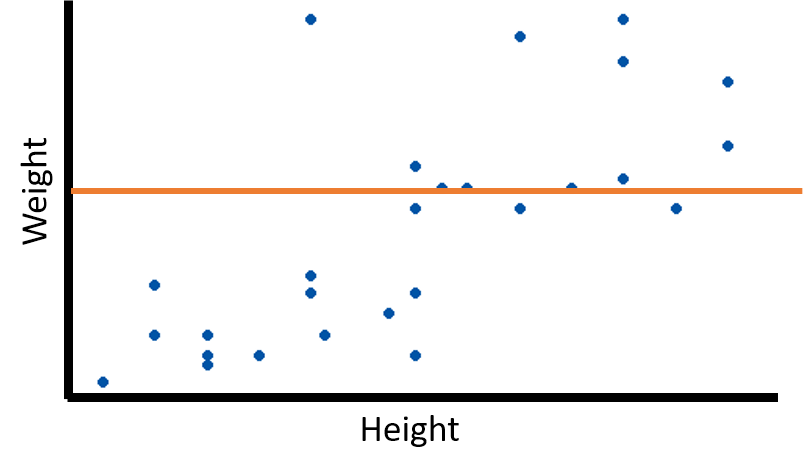
\includegraphics[scale=0.4]{img/underfit.png}
		\caption{Underfitting~\cite{gs}}
		\label{fig:underfit}
	\end{figure}
	\Cref{fig:underfit} shows that for any point in the diagram, the function always assigns the same predicted value. Solving the problem of underfitting means making the line approximate the data better.
	\item \textit{Overfitting:} 
	\begin{figure}
		\centering
		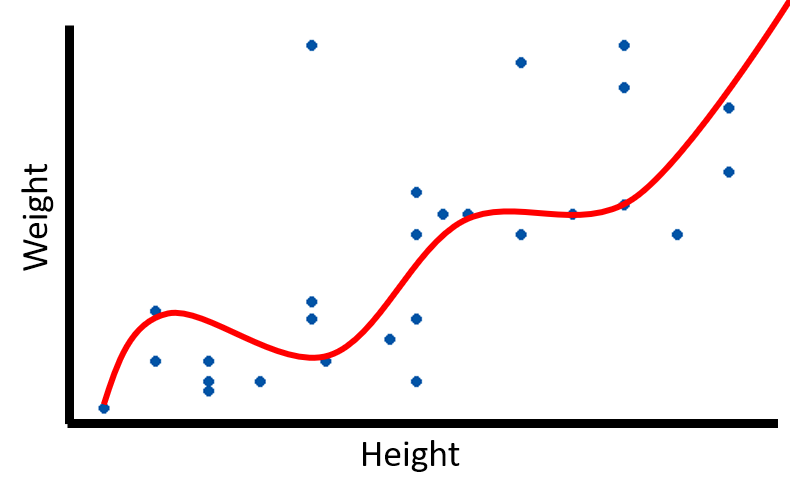
\includegraphics[scale=0.4]{img/overfit.png}
		\caption{Overfitting~\cite{gs}}
		\label{fig:overfit}
	\end{figure}
	\Cref{fig:overfit} shows that for any point in the diagram, the function performs very good. However, the function has become very inflexible and it will not perform good enough on new points. According to~\cite{tfidf}, overfitting can also be understood as a probable distribution of data. The training set of data that the line is being drawn through is just a sample of a larger unknown set, and the line which will be drawn needs to fit the larger set equally well if it is to have any predictive power. Therefore, it must be assumed that our sample is loosely representative of a larger set.
\end{itemize}
Another field of Artrificial Intelligence is~\ac{nlp}, which provides tools for analyzing and deriving meaning in human language. To do so,~\ac{nlp} provides a means to process lexical properties as well as syntactic recognition of the human language. However, human language can be rarely precise and ambiguous. Even though~\ac{nlp} has a very wide range of applications, such as automatic text summarizing, relationship extracting, stemming, sentiment analysis and more, it is a difficult problem to tackle in computer science.

\subsection{Sklearn}
\subsubsection{Definition}
Sklearn (a.k.a scikit-learn) is defined \footnote{http://scikit-learn.org/stable/} as a simple and efficient set of tools for data mining and data analysis. It is built on NumPy and SciPy. Sklearn will provide not only the classifiers needed for the pipeline but also meaningful tools.
\subsubsection{Application}
Sklearn has provided the following tools for this project:
\begin{itemize}
	\item \textit{Train and Test splitting}: This method is responsible for splitting the main dataset into two parts, one for training the model and the other one for testing the model. It is a very common~\ac{ml} technique. In addition, the testing set will later be used to compute parameters such as accuracy and f1 score. More information on accuracy and f1 score can be found in \cref{sec:score}.
	\item \textit{Pipeline}: A pipeline is a set of procedures connected in series, one after the other where the output of one process is the input to the next~\cite{pipeline1}. Image~\ref{fig:pipeline}\footnote{\url{https://www.slideshare.net/databricks/dataframes-and-pipelines}} represents the idea of a pipeline, though it does not resemble exactly this projects' pipeline.
	\item \textit{\acl{tfidf}}: The~\acf{tfidf} is used for every word. It contains two parts; the \textit{if} part, which represents the word frequency and the \textit{idf} part, which represents inverse document frequency~\cite{tfidf1}. This term represents a words' weight in a text.
	\item \textit{Count Vectorizer}: The algorithm consists of representing a token by considering how many times it appears in a text~\cite{countvect1}. It basically counts the vocabulary and generates a dictionary which can later be fed into a pipeline, like in this project.
	\item \textit{\acl{nb}}: A multinomial distribution useful to model feature vectors where each value represents a number of occurrences of a term (or its relative frequency)~\cite{countvect1}.
	\item \textit{\acl{svm}}: Given a set of training examples, each marked as belonging to one or the other of two categories, a \acf{svm} training algorithm builds a model that assigns new examples to one category or the other, making it a non-probabilistic binary linear classifier\footnote{\url{https://en.wikipedia.org/wiki/Support_vector_machine}}.
	\item \textit{\acl{knn}}: Is a non-generalized~\ac{ml} algorithm that computes distances from one point to all the training dataset points and chooses the $k$ nearest points~\cite{countvect1}.The KNeighbors classifier has been fed into the pipeline as input.
	\item \textit{\acl{lr} classifier}: Is analogous to multiple linear regression, except the outcome is binary. Various transformations are employed to convert the problem to one in which a linear model can be fit~\cite{lr1}.
\end{itemize}

\begin{figure}
	\centering
	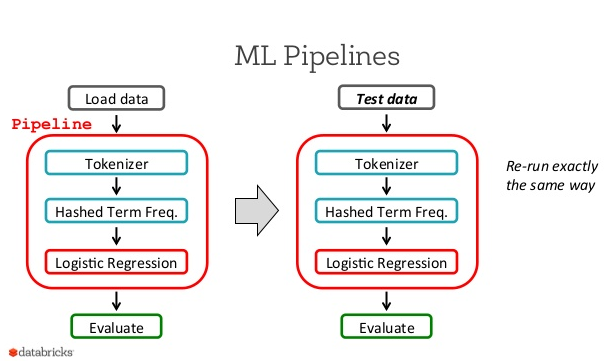
\includegraphics[width=\linewidth]{img/pipeline1.png}
	\caption{A Pipeline.~\cite{pipeline}}
	\label{fig:pipeline}
\end{figure}

All the methods illustrated above are widely explained altogether with an implementation clarification in~\cref{sec:clasif}.
\section{Senpy}
Senpy~\cite{senpy} is a framework for text analysis using linked data. It aims at providing a framework where analysis modules can be easily integrated as plugins and, at the same time, provides the core functionalities (data validation, user interaction, logging, etc).

\subsection{Architecture}
Senpy introduces a modular and dynamic architecture which allows implementing different algorithms in an extensible way while offering a common interface and offering common services that facilitate development, so developers can focus on implementing new and better algorithms.\par
To do so, the architecture consists of two main modules:
\begin{itemize}
	\item Senpy core: Building block of the service.
	\item Senpy plugins: Analysis algorithms.
\end{itemize}
\begin{figure}
	\hspace{-2.1cm}
	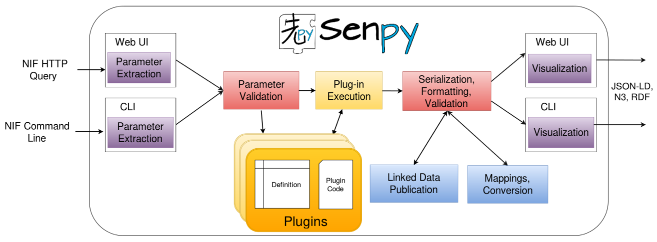
\includegraphics[scale=0.85]{img/senpy_architecture.png}
	\caption{Senpy's Architecture~\cite{senpy}}
	\label{fig:senpyarch}
\end{figure}
\Cref{fig:senpyarch} depicts a simplified version of the processes involved in Senpy analysis framework.

\section{Bitter}
\label{sec:bitter}
In order to download the Tweets which integrate partially the dataset, the tool bitter was used. Bitter is able to automate several actions (e.g. downloading Tweets) by using a Python wrapper over Twitter which adds support for several Twitter API actions~\footnote{https://github.com/balkian/bitter}.\\
Bitter could be used after installing it and running commands on the UNIX terminal.
\subsection{Architecture}
\Cref{fig:bitter} explains how was bitter used in this project. On the left, the reader can see the information provided to the bitter tool. The configuration file is needed to download the tweets, otherwise, nothing will be downloaded. The file contains the user credentials for accessing the Twitter database.\\ The tweet id file is a \textit{.csv} database containing in one column the desired tweets. Finally, bitter will download in \textit{.json} format all the tweets in the indicated folder (indicated on the command). For those tweets that, by any reason, could not be downloaded, a folder named \textit{error} will be created containing the tweet ids that failed.
\begin{figure}
	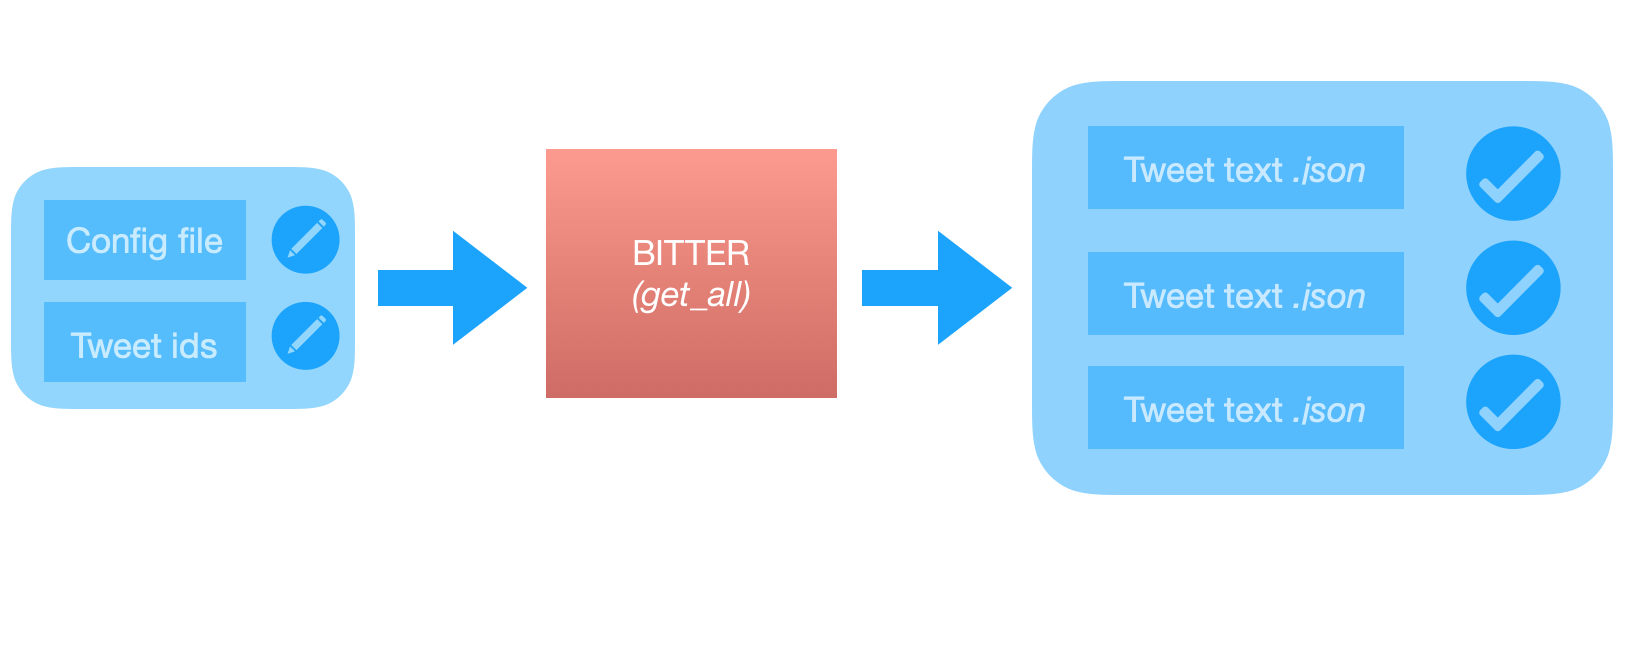
\includegraphics[width=\linewidth]{img/bitter.png}
	\caption{Bitter Architecture}
	\label{fig:bitter}
\end{figure}
\section{Elasticsearch}
Elasticsearch is a highly scalable open source search engine with a very powerful analytical engine. The data stored in Elasticsearch is \ac{json} formatted. The primary way of interacting with Elasticsearch is via \textbf{REST API}~\cite{elastic1}. The most powerful tool that Elasticsearch provides is indexing. Indexing becomes a very important task when dealing with lots of amount of data, in this case, with many tweets.
\subsection{Architecture}
All data stored in Apache Lucene's data is stored in \textit{inverted index}. This means that the data is being transformed. The process of transforming data is called analysis, which relies in two basic pillars: \textbf{tokenizing} and \textbf{normalizing}. The normalizing step is mandatory to make the tokens readable. Inverted index processes are performed by analyzers. An analyzer is composed of a tokenizer and one or more token filters. During the indexing time, when Elasticsearch processes a field that must be indexed, it checks whether an analyzer is defined in several levels~\cite{elastic1}.\\
When it comes to indices, Elasticsearch uses shards and replicas in order to distribute data around the cluster.\\
Elasticsearch distributes the shards by performing a process called \textit{sharding}. The indices (or index) are called shards and Elasticsearch automatically manages the shards, like a low-level working unit.
\begin{figure}
	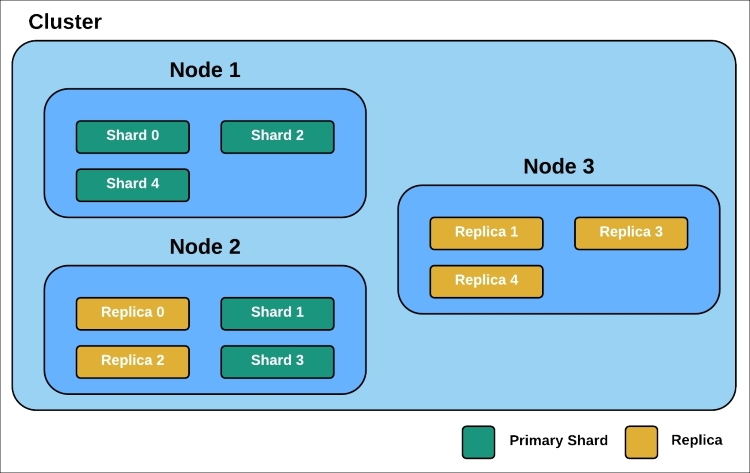
\includegraphics[width=\linewidth]{img/elasticsearch.jpeg}
	\caption{Elasticsearch~\cite{elastic3}}
	\label{fig:elastic1}
\end{figure}
The most common terms used in Elasticsearch are:
\begin{itemize}
	\item \textit{Node}: An instance of Elasticsearch running on a machine.
	\item \textit{Cluster}: The name under which one or more nodes are connected.
	\item \textit{Document}: A \ac{json} object containing the actual data in key-value pairs.
	\item \textit{Index}: Logical namespace in which Elasticsearch stores data.
	\item \textit{Doc types}: A class of similar documents. A type consists of a name and a mapping.
	\item \textit{Shard}: Containers which can be stored on a single node or multiple nodes. A  shard can be either primary or secondary. A primary shard is the one where all the operations that change the index are directed. A secondary shard is the one that contains duplicate data of the primary shard and helps in quickly searching the data as well as for high availability; in a case where the machine that holds the primary shard goes down, then the secondary shard becomes the primary automatically.
	\item \textit{Replica}: Duplicate copy of the data living in a shard for high availability.
\end{itemize}
Finally, as mentioned before, Elasticsearch can be related to a traditional database managing system. This is depicted in~\Cref{fig:elastic2}.
\begin{figure}
	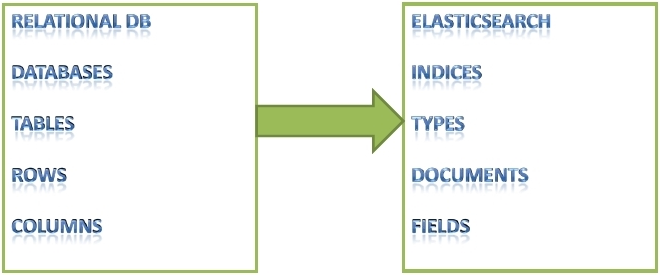
\includegraphics[scale=0.65]{img/elastic_1.png}
	\caption{Elasticsearch and a Database~\cite{elastic1}.}
	\label{fig:elastic2}
\end{figure}
\section{Pickle}
The pickle module makes it possible to store an object in a file in a standard format for later use by the same or a different program. The stored can be any type of object as long as it does not require an operating system resource such as a file handle or network socket~\cite{pickle}.\\
Pickle is very useful for using an already trained classifier in different modules.





	\chapter{Requirement Analysis}
\label{chap:use-case}

\section{Introduction}
\label{sec:introduction}
\section{Use cases}
\label{sec:use-cases}

\subsection{System actors}
\label{subsec:system-actors}
	\chapter{Architecture}
\label{chap:architecture}


\section{Introduction}
\label{sec:introduction}
In this chapter, we cover the design phase of this project, as well as implementation details involving its architecture. Firstly, we present an overview of the project, divided into several modules. This is intended to offer the reader a general view of this project architecture. After that, we present each module separately and in much more depth.


%\newpage

	\chapter{Case study}
\label{chap:case-study}

\section{Introduction}
\label{sec:introduction}
In this chapter we are going to describe a selected use case. This description will cover the main Wool features, and its main purpose is to completely understand the functionalities of Wool, and how to use it. 
\section{Rule edition}
...
	\chapter{Conclusions and future work}
\label{chap:conclusions}
The conclusions reached in the previous chapter will be brought together in this chapter.\\
Moreover, a description of the achieved goals and the lines of future work will be explained.\\
Finally, the problems faced will be presented.

\section{Conclusions}
\label{sec:conclusions}
This project resembles an example of automatic sarcasm detection. The approach followed was training a classifier using a dataset consisting of two columns, one for the text body and the last column to feature the sarcastic property of the text body. This goal was fulfilled by making use of~\ac{ml} techniques and~\ac{nlp} techniques, with the ability to detect sarcasm in short text, such as Twitter.\\
To compile the final dataset, three datasets containing tweets where assembled and put together generating a final dataset with the tweet body and the feature.\\
Later on, the model could be built by introducing a preprocessing stage designed to encode categorical variables and delete tweets lacking a text body. To ensure a non-dependency between the tweets, the rows of the dataset were randomized.\\
Once the dataset was ready a pipeline was designed, which would be responsible for the feature extraction process. The features that gave more information to the classifier were:
\begin{enumerate}
	\item \textbf{Lexical features:} The word repetition frequency had a relationship with the sarcastic property of a short text.
	\item \textbf{Ngram features:} This feature shows that depending on how many words uses the algorithm to consider a noun, the model can be more precise.
	\item \textbf{Number of topics feature (\ac{lda}):} Taking into account the possible number of topics that a text can be talking about is a relevant characteristic of sarcasm.
\end{enumerate} 
As an interesting fact, the model predicted with more accuracy having only these three features extracted rather than counting on the syntactic features.\\
The next step was to feed the features extracted to a classifier. According to~\cite{clasif}, a classifier is a kind of rule-based system with general mechanisms for processing rules in parallel, for adaptive generation of new rules, and for testing the effectiveness of new rules. The classifiers which had an outstanding performance were:
\begin{enumerate}
	\item \textbf{\acl{nb}}: This classifier was by far the best one, reaching an F1 score of $0.92$.
	\item \textbf{\acl{lr}}: This classifier had an F1 score of $0.91$.
	\item \textbf{\acl{svm}:} This classifier had an F1 score of $0.91$.
\end{enumerate} 
The three classifiers were trained using a training set and the F1 score was extracted by using a testing set.
Additionally, the~\acl{knn} classifier was also implemented but it had a very bad performance.\\
Finally, the senpy engine was implemented to provide a user-friendly interface allowing the user to insert text and get a message saying if the tweet is sarcastic. An example can be found in~\Cref{fig:senpyex1}.

\section{Achieved goals}
The main goals achieved in this project were:
\begin{description}
	\item \textbf{Construction of a~\ac{ml} classifier capable of detecting sarcasm in short texts, such as tweets.}\\
	This was the main objective of this project.
	\item \textbf{Implementation of the classifier in a web engine which allows any user to detect sarcasm in a user-inserted text.}\\
	This goal could be achieved because of the Senpy engine.
	
\end{description}

\section{Future work}
In regard to the future development of the model, the following improvements could be done:
\begin{enumerate}
	\item More feature detection. In sum, only four features have been extracted in this project, however, more features could give more information concerning sarcasm. However, this classifier has shown a better performance when analyzing three features rather than four. Therefore, if many more features are considered, the performance of the classifier may be degraded due to the overfitting phenomenon.
	\item Take into account previous tweets. It is very common that tweets are used to answer other tweets. Sometimes the sarcasm is hidden in an answer to a message. In this project, that possibility was never considered, deeming a sarcastic tweet only if the tweets' text field is sarcastic. It could be a good improvement to consider the text field of a tweet and also the predecessing tweets' text field.
	\item Implement a dashboard. In~\cref{sec:elastic} it was discussed the possibility of using the elastic search engine to generate a dashboard and offer a better interface to the user. To do so, the Sefarad engine offered by the Intelligent Systems Group at the UPM (GSI) is very useful. In~\cite{sefarad} more information regarding the dashboard can be found.
\end{enumerate}
\section{Problems encountered}
The problems faced in this project shall be explained
\begin{enumerate}
	\item \textbf{Technologies used}: At the beginning of the project, it was required that I learned all the technologies used as well as the libraries implemented. This required a considerable amount of time.
	\item \textbf{Retrieval of tweets:} The provided datasets contained only a column indicating the tweet id and sarcastic value ('True' or 'False'). To retrieve the text bodies that would later be fed to the classifier, those text bodies were obtained by using the Bitter(\cref{sec:bitter}) software. 
	
\end{enumerate}



	
	
	
	\appendix
	
	\phantomsection
	\nocite{*}
	\addcontentsline{toc}{chapter}{Bibliography}
	%ieeetr
	\bibliographystyle{plain}
	{
	\small
	\bibliography{biblio/ref}
	}
	%\cleardoublepage
	\end{document}